\documentclass{ctexart}
\usepackage{graphicx}
\usepackage{amsmath}
\usepackage{amsthm}
\usepackage{amssymb}
\usepackage{fancyhdr}
\usepackage{ifthen}
\usepackage{syntonly}
\usepackage[colorlinks, CJKbookmarks=true, linkcolor=red]{hyperref}
\pagestyle{plain}
\usepackage[raggedright]{titlesec}
\newtheorem{性质}{性质}
\newtheorem{定理}{定理}
\newtheorem{推论}{推论}
\begin{document}
\title{作业}
\author{计算机科学与技术系52班 杨定澄 \and 学号:2015011274 \and E-mail:892431401@qq.com}
\date{}
\maketitle
\section{第一题}
可以在HMM.py中看到程序。

\subsection*{(1)}

先看第一问,假设$n$代表显状态数目(ABCD,共$4$个),$m$代表隐状态数目($3+2$,共$5$个。初始节点为$0$,终止节点为$4$)。我们要根据已知的样本学习$A$矩阵与$B$矩阵,其中$A_{ij}$代表第$i$个隐状态到第$j$个隐状态的转移概率,$B_{ij}$表示第$i$个隐状态发射出第$j$个显状态的概率。接着套用书上的Baum-Welch算法。

但是这时我们遇到了第一个问题,书上的算法是基于给定一个样本输出$O$,来学习一个参数$\theta$,使得$P(\theta|O)$最大的,这里有一组样本。我分别在两个模型中各取一个样本进行学习。

接着考虑我们要学习的是哪些量,因为有的量是固定的,比如$A_{i0}=0,A_{44}=1$。

所以一开始我的做法是,隐状态$0,1,2,3$等概率的转移到隐状态$1,2,3,4$,然后每个隐状态对显状态的发射概率是等概率的,接着让他学习。学习结果如下

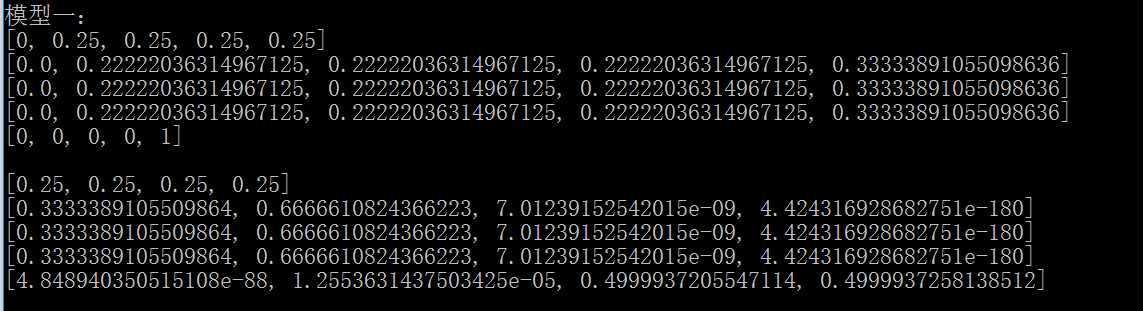
\includegraphics[width=6in,height=4in]{1.png}


对于每个模型,第一个矩阵是$A$矩阵,第二个矩阵是$B$矩阵。结果相当令人诧异,可以看出最后会很快的跑到隐状态的终止节点,让他生成剩下的串。一般会有某个字符几乎百分之百的由终止节点隐状态生成。比如模型一训练的样本是AABBCCDD,就变成了AABB由前$4$个隐状态生成,后面的CCDD几乎百分之百的由终止状态生成。

产生这种现象的原因之一,可能还是在于串长不够长、隐状态数大于显状态数,导致了某个字符几乎完全由某组隐状态生成的分工现象。

题目要求是串从起始状态出发,终止状态结束。为了让终止状态的“终止”意义更大,我觉得要求只有第一个字符由起始节点生成、只有最后一个字符由终止节点生成更加合适,所以我将程序改了一下,强制要求只有最后一个字符才能由终止状态生成。

要想做到这一点,我们可以修改forward-backward算法,也就是在dp的时候要求只有最后一个字符才能走到隐状态上去。如此一来,学习的结果就会变成我想要的结果了。

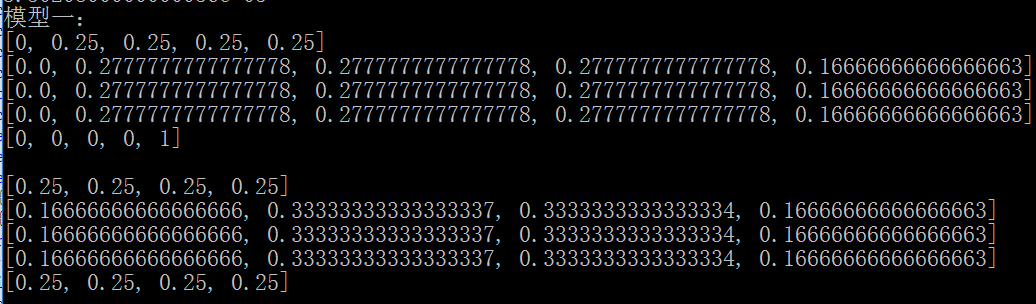
\includegraphics[width=6in,height=4in]{2.png}

接着在两组样本中各取第一个样本进行训练,却又遇到了一个问题。

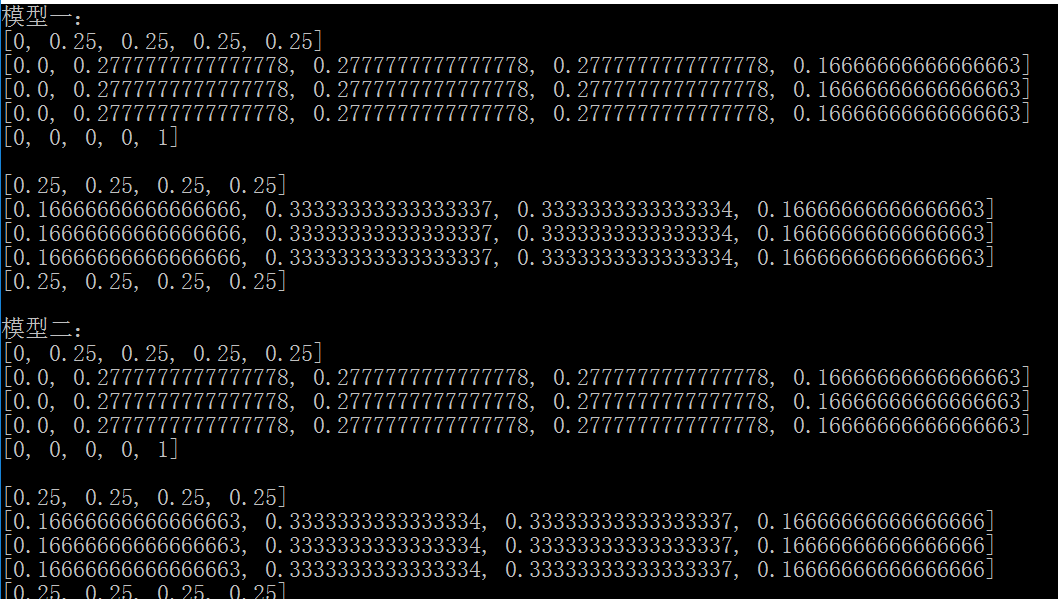
\includegraphics[width=6in,height=4in]{3.png}

可以看出,训练的结果几乎一模一样。

观察发现,我们训练的两个样本分别是AABBCCDD,DDCCBBAA,事实上他们只是被置换了一下而已,其实是很像的两个串。

更关键的是,我的初始值设定的是均匀分布(即都是0.25),这么一来算法对这两个串的运行结果都会是一样的。

事实上,如果两个训练模型的初始值设定一样,对这两个串训练出来的结果也都会是一样的。

为此,我们可以修改初始值,比如第一个样本不是均匀分布而是$[0.1,0.2,0.3,0.4]$,第二个正好相反,是$[0.4,0.3,0.2,0.1]$,这样子设定初始值得到的训练结果就有所不同了。

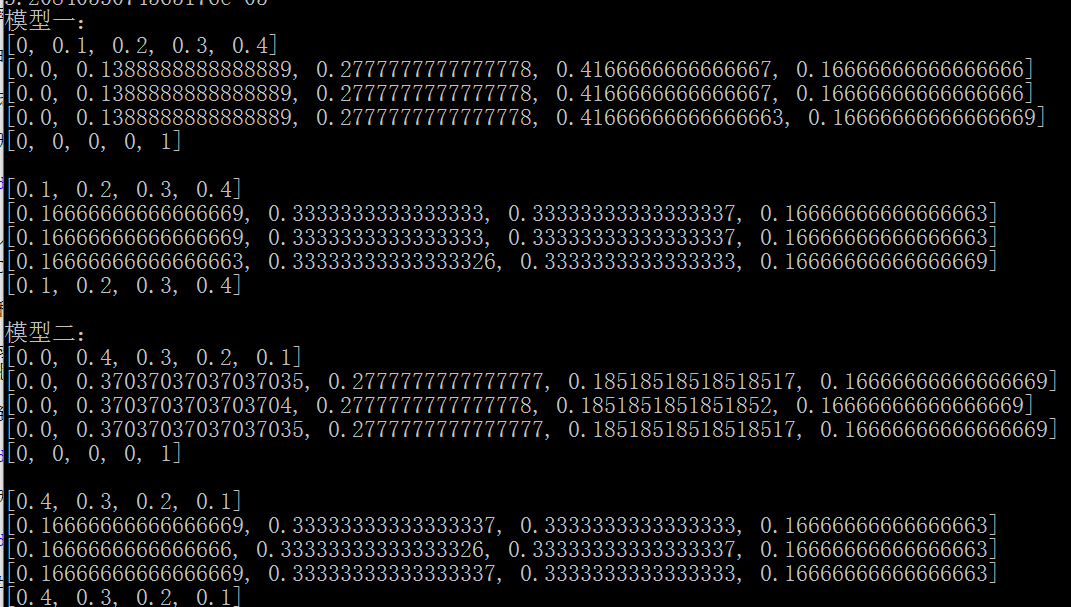
\includegraphics[width=6in,height=4in]{4.png}

而如果选择的样本不这么相似,比如第二组样本使用的是DDABCBA,则训练出来的结果就会有更明显的不同。

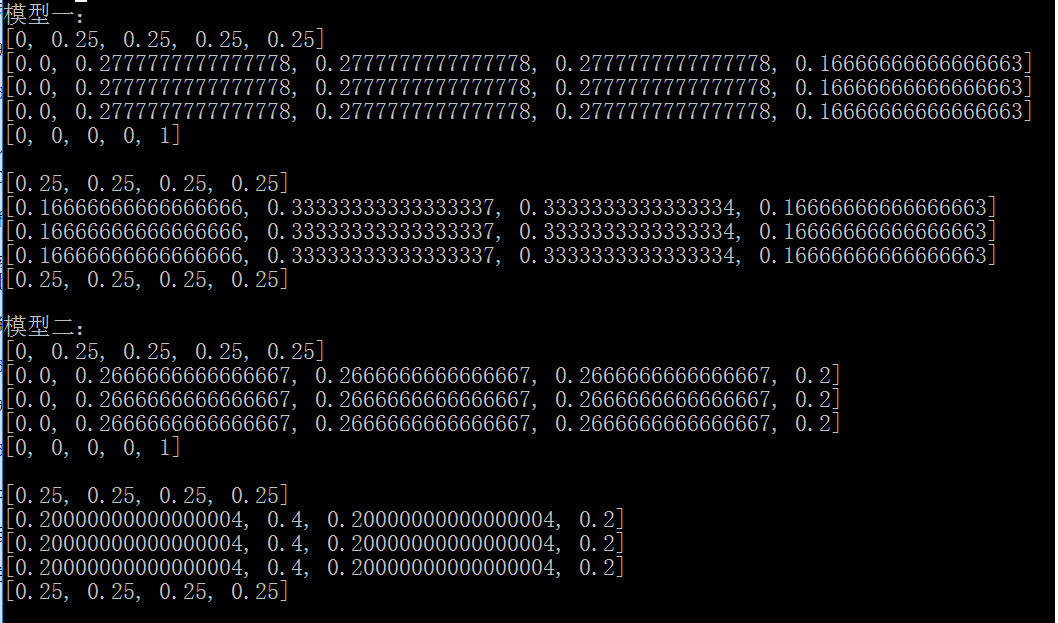
\includegraphics[width=6in,height=4in]{5.png}

从中可以看出,初始值的选定是相当重要的,两个比较相似的串,如果初始值一样,很容易收敛到同一个解,从而得到相同的模型,这是我们极力要避免的。

一个最简单的避免方法是初始值随机选定。
\subsection*{(2)}
解决了第一问后,后两问就相当简单了。

隐马尔可夫模型的三大核心问题里,后两问其实都是估值问题,而估值问题可以说是学习问题的一个步骤,所以几乎不用写什么新代码。

第一个模型学习样本AABBCCDD,第二个模型学习样本DDABCBA,生成给定的四个串概率和分类如下:

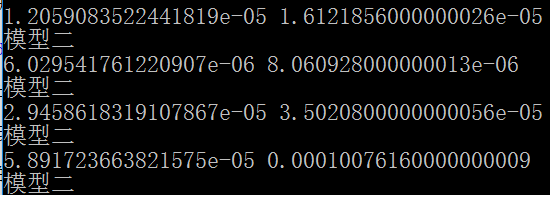
\includegraphics{6.png}

生成的四个串全都被分类到了第二类,这点令我感到惊讶。

直观上来看,第一个样本AABBCCDD未免过于规律,而DDABCBA则显得更加像随机生成的,同时又有“相邻两个字符相同”的情况出现。

从概率数值上看,对于前三个,虽然都分给了第二类,但其实概率相差的也不算太大。

如果第一个样本换成一个更加随机一点的,分类结果就不会这么一边倒了。(反之如果一个样本全部都是A,那么基本上不会有什么串和他一类)

\subsection*{(3)}

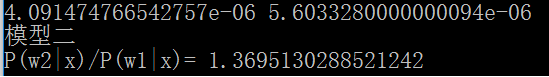
\includegraphics{7.png}

可以对$\frac{P(\omega1)}{P(\omega_2)}$以$1.3695$为分界点,当比值恰好取在分界点上时后验概率可视为一样。

如果$\frac{P(\omega1)}{P(\omega_2)}>1.3695$,倾向于分在第一类,否则倾向于分在第二类。
\section{第二题}
\subsection*{(1)}
贝叶斯置信网络相当于是所有变量按照“依赖关系”形成一个有向无环图,我们假设对一个长度为$T$的串用一阶马尔科夫模型,那么我们把时刻$t$所在的隐状态设为一个变量。

如此一来,由于时刻$t$所在的隐状态只和时刻$t-1$所在的隐状态有关,故形成一个有向无环图。

即时刻$t$对应变量向时刻$t+1$对应变量连一条边。

贝叶斯置信网络的公式为$P(x|e) \propto P(e^C|x)P(x|e^P)$,我们来思考$P(x|e^P)$是什么。

根据贝叶斯置信网络

\[
P(x|e^P)=\sum_{all i,j,\cdots,k} P(x|P_{1i},P_{2j},\cdots,P_{|P|k})P(P_1|e_{p_1})\cdots P(P_{|P|_k}|e_{P_{|P|_k}})
\]

$P_{mn}$表示的就是$P_m$取$n$的概率。

由于每个变量只有最多一个父亲(就是前一个时刻对应变量),所以应用在马尔科夫过程就是

\[
P(x|e^P)=\sum_{i} P(x|P_{1i})P(P_1|e_{p_1})
\]

假设$x$集合只有一个变量$x_i$,我们会发现$P(x_i=j|e^P)$表达就是只考虑$x_i$的父亲的情况下,$x_i=j$的概率。而这其实就是前向算法中的$\alpha$数组。

前向算法中$\alpha_i(t)$表示时刻$t$处于隐状态$i$,意思就是时刻$t$对应的变量取值为$i$的概率,也就是$P(x_t=i|e^P)$。

前向算法的转移式为$\alpha_i(t)=\sum_j \alpha_j(t-1)a_{ij}b_{jk}v(t)$,其中$\alpha_j(t-1)$就代表$P(P_1|e_{p_1})$这一项,$a_{ij}b_{jk}v(t)$就代表$P(x|P_{1i})$这一项。

而当$t=0$时,自然是$P(x_0=\textrm{初始状态}|e^P)=1,P(x_0=\textrm{初始状态以外状态}|e^P)=0$。

所以前向算法得证。

后向算法其实是前向算法的逆过程,我们可以改改变量的含义。假设有$T$个时刻,就对应的有$T$个变量,第$i$个变量取值为$j$的意思是,我现在在时刻$i$,处于隐状态$j$,最后时刻$T$的时候我会处于终止状态。这样就得到了$T$个状态。

这么一来的话,每个状态就不是和前面的状态有关了,而是和后面的状态有关,时刻$t$对应变量依赖于时刻$t+1$对应变量。

接着假设$x$集合只含有一个变量$x_i$,$P(x|e^P)$就是$\beta_i(t)$的含义了。$P(P_1|e_{p_1})$对应的是$\beta_j(t+1)$,$a_{ij}b_{jk}v(t+1)$代表$P(x|P_{1i})$这一项
\subsection*{(2)}
基本上如上问所说。

对于隐马尔可夫模型,假设一个时间为$T$的序列,总共有$m$个隐状态。

我们可以看做有恰好$T$个变量,$x_i$表示时刻$i$所处的隐状态编号,$1 \le x_i \le m$。

对于$i>0$,$x_i$依赖且仅依赖于$x_{i-1}$。$x_0$没有依赖的变量。

注意依赖关系构成一个有向无环图的形式,所以也是一个贝叶斯置信网络的应用。
\end{document}
